\documentclass[12pt, letterpaper]{article}
\usepackage[utf8]{inputenc}
\usepackage{geometry}
\geometry{margin=1in}
\usepackage{graphicx}
\usepackage{float}
\usepackage{booktabs}
\usepackage{amsmath}
\usepackage{caption}
\usepackage{subcaption}
\usepackage{xcolor}
\usepackage{tcolorbox}
\usepackage{tikz}
\usetikzlibrary{shapes, arrows, positioning, calc}
\usepackage{circuitikz} % Try to use if available, otherwise fallback to tikz
\usepackage{listings}
\usepackage{array}
\usepackage{titlesec}
\usepackage{fancyhdr}
\usepackage{hyperref}
\usepackage[nameinlink,noabbrev]{cleveref}

% --- Caption formatting ---
\captionsetup{
  font=small,
  labelfont=bf,
  labelsep=period,
  justification=centering,
  singlelinecheck=false,
  skip=6pt
}
\captionsetup[table]{position=top}

% --- Section headings ---
\titleformat{\section}{\Large\sffamily\bfseries}{\thesection}{0.6em}{}
\titleformat{\subsection}{\large\sffamily\bfseries}{\thesubsection}{0.5em}{}
\titleformat{\paragraph}[block]{\normalfont\normalsize\bfseries}{}{}{}
\titlespacing*{\section}{0pt}{1.2ex plus .3ex}{0.6ex}
\titlespacing*{\subsection}{0pt}{1.0ex plus .2ex}{0.4ex}
\titlespacing*{\paragraph}{0pt}{0.8ex}{0.6ex}

% --- Header / footer ---
\newcommand{\coursenum}{MECH 421}
\newcommand{\labnum}{Lab 5}
\newcommand{\labtitle}{PCB Assembly and Stepper Motor Control}
\newcommand{\studentone}{Gyan Edbert Zesiro}
\newcommand{\studentoneid}{38600060}
\newcommand{\studenttwo}{Ryan Edric Nashota}
\newcommand{\studenttwoid}{33508219}
\newcommand{\labperformed}{7~November~2025}
\newcommand{\labsubmitted}{28~November~2025}
\pagestyle{fancy}
\fancyhf{}
\lhead{\sffamily \labnum}
\chead{\sffamily \labtitle}
\rhead{\sffamily Gyan, Ryan}
\renewcommand{\headrulewidth}{0.4pt}
\cfoot{\sffamily \thepage}
\setlength{\headheight}{15pt}
\addtolength{\topmargin}{-3pt}

% --- Cleveref ---
\Crefname{figure}{Figure}{Figures}
\Crefname{table}{Table}{Tables}
\Crefname{equation}{Equation}{Equations}
\Crefname{section}{Section}{Sections}
\crefname{figure}{figure}{figures}
\crefname{table}{table}{tables}
\crefname{equation}{equation}{equations}
\crefname{section}{section}{sections}

% --- Graphics path ---
\graphicspath{{../analysis_outputs/figures/}{figures/}}
\newtcolorbox{infobox}[1][]{colback=blue!5,colframe=cyan!60!black,title=#1,boxrule=0.6pt}

% --- Code listing style ---
\definecolor{codegreen}{rgb}{0,0.6,0}
\definecolor{codegray}{rgb}{0.5,0.5,0.5}
\definecolor{codepurple}{rgb}{0.58,0,0.82}
\definecolor{backcolour}{rgb}{0.95,0.95,0.92}

\lstdefinestyle{mystyle}{
    backgroundcolor=\color{backcolour},
    commentstyle=\color{codegreen},
    keywordstyle=\color{magenta},
    numberstyle=\tiny\color{codegray},
    stringstyle=\color{codepurple},
    basicstyle=\ttfamily\footnotesize,
    breakatwhitespace=false,
    breaklines=true,
    captionpos=b,
    keepspaces=true,
    numbers=left,
    numbersep=5pt,
    showspaces=false,
    showstringspaces=false,
    showtabs=false,
    tabsize=2
}
\lstset{style=mystyle}

% --- Placeholder command for images ---
\newcommand{\imageplaceholder}[2]{
    \begin{figure}[H]
        \centering
        \fbox{\begin{minipage}{0.8\textwidth}
            \centering
            \vspace{2cm}
            \textbf{PLACEHOLDER FOR: #1} \\
            \vspace{1cm}
            \textit{#2}
            \vspace{2cm}
        \end{minipage}}
        \caption{#1}
        \label{fig:#1}
    \end{figure}
}

% --- Title block ---
\makeatletter
\renewcommand{\maketitle}{
  \vspace*{1ex}
  \begin{center}
    {\sffamily
      {\Large \coursenum\ --- \labnum\par}
      \vspace{0.6ex}
      {\huge \bfseries \labtitle\par}
      \vspace{0.8ex}
      {\large \studentone\enspace (ID:\ \studentoneid) \\[0.4ex]
      \studenttwo\enspace (ID:\ \studenttwoid)\par}
      \vspace{0.6ex}
      {\normalsize Lab Performed:\ \labperformed \\ 
      Report Submitted:\ \labsubmitted\par}
    }
  \end{center}
  \vspace{1.2ex}
  \thispagestyle{empty}
}
\makeatother

% --- Body spacing ---
\setlength{\parindent}{0pt}
\setlength{\parskip}{0.6em}

% --- Metadata ---
\title{\coursenum\ \labnum\\\labtitle}
\author{\studentone\ (ID:\ \studentoneid) \\ \studenttwo\ (ID:\ \studenttwoid)}
\date{}

\begin{document}
\pagenumbering{gobble}
\maketitle

\begin{abstract}
This lab focused on building and testing a PCB designed to control stepper, and DC motors
through microprocessor commands, though for this lab we are only focusing on 
stepper motors. The lab was completed in three main sections. 
First, we assembled and soldered the PCB, verifying proper functionality of the power supply, USB interface, microprocessor, 
and motor driver components. We configured UART communication to enable data transfer for 
future exercises. Second, we developed firmware to control a stepper motor using half-stepping, 
implementing both single-step commands and continuous velocity control through a C\# graphical interface. 
We measured the maximum loaded and unloaded speeds of the motor and analyzed the factors limiting its performance. 
Finally, we expanded the system to control a two-axis gantry stage using dual stepper motors. We programmed the microcontroller 
to execute coordinated movements, allowing the stage to follow straight-line paths between specified coordinates. 
The system successfully drew predetermined shapes and a custom design, demonstrating precise synchronized control of both axes. 
Throughout the lab, we gained practical experience in PCB assembly, firmware development, serial communication protocols, 
and motion control algorithms while exploring the advantages and limitations of stepper motors for precision positioning applications.
\end{abstract}

\clearpage
\pagenumbering{roman}
\setcounter{page}{1}
\renewcommand{\contentsname}{Table of Contents}
\tableofcontents
\clearpage
\renewcommand{\listfigurename}{Table of Figures}
\listoffigures
\clearpage
\listoftables
\clearpage
\setcounter{tocdepth}{2}
\pagenumbering{arabic}
\setcounter{page}{1}
\pagestyle{fancy}

\section{Introduction}
The purpose of this lab is to gain hands-on experience in PCB assembly, soldering surface-mount components, and 
implementing real-time control for stepper motors using a microcontroller. 
The final system is a 2-axis gantry capable of drawing complex shapes, demonstrating the integration of hardware 
(PCB, motors, mechanics) and software (firmware, PC interface).

\section{Exercise 1: PCB Assembly and Soldering}

\subsection{Objective}
The goal of this exercise is to populate a bare PCB with surface-mount and through-hole components to create a 
functional motor control board. This board includes a microcontroller (MSP430), USB interface (FTDI), power regulation, 
and motor drivers. This exercise also teaches us how to solder SMD components and troubleshoot common issues.

\subsection{Circuit Description}
The PCB consists of several key functional blocks:
\begin{itemize}
    \item \textbf{Power Supply}: Converts external 12V DC input to 5V and 3.3V logic levels using linear regulators (NCP1117). 5V is used for the USB interface and some logic, while 3.3V powers the MSP430 microcontroller.
    \item \textbf{USB Interface}: Uses an FT230XS chip to convert USB signals from a PC into UART (Serial) signals compatible with the microcontroller. This allows for data logging and control commands.
    \item \textbf{Microcontroller}: The MSP430FR5739 is the brain of the board. It executes firmware to generate PWM signals for motors, read sensors, and communicate via UART.
    \item \textbf{Motor Driver}: The DRV8841 is a dual H-bridge driver capable of driving DC motors or bipolar stepper motors. It handles the high currents required by the motors, controlled by low-power logic signals from the MCU.
\end{itemize}

\subsection{Parts List}
The following components are required for assembly. Ensure all parts are accounted for before starting.

\begin{table}[H]
\centering
\begin{tabular}{@{}>{\raggedright\arraybackslash}p{4.6cm}%
                >{\raggedright\arraybackslash}p{6.7cm}%
                >{\centering\arraybackslash}p{1.5cm}%
                >{\centering\arraybackslash}p{1.0cm}@{}}
\toprule
\textbf{Reference} & \textbf{Description} & \textbf{Source} & \textbf{Qty} \\ \midrule
5x1 header programming & Bergstik II 0.100" straight header & Kit & 1 \\
Motor bypass cap & 1000\,$\mu$F 50V 20\% alum SMD & Kit & 2 \\
MCU core bypass & 0.47\,$\mu$F 16V 5\% X7R 0603 & Kit & 1 \\
0.01\,$\mu$F charge pump critical & 10{,}000\,pF 100V 5\% NP0 1206 & Kit & 1 \\
51\,pF filter encoder & 51\,pF 50V 5\% NP0 1206 & Kit & 2 \\
20-pin MCU header & 20\,pos 0.100" straight header & Kit & 2 \\
DC wall jack & 2.1\,mm PCB power jack & Kit & 1 \\
USB connector & Mini-USB receptacle, 5\,pos & Kit & 1 \\
PSU diode & Schottky diode 40V 3A DO-214AC & Kit & 2 \\
Polyfuse USB & Resettable fuse 6V 0.50A 1206 & Kit & 1 \\
Latch & Dual D-type latch, 14-SOIC & Kit & 2 \\
Inverter & Hex Schmitt-trigger inverter, 14-SOIC & Kit & 2 \\
3.3V PSU & LDO regulator 3.3V 1A SOT-223 & Kit & 1 \\
5.0V PSU & LDO regulator 5V 1A SOT-223 & Kit & 1 \\
USB chip (FT230XS) & USB serial basic UART 16-SSOP & Kit & 1 \\
Green LED & Green LED clear 1206 SMD & Kit & 6 \\
Current sense resistors & 0.2\,$\Omega$ 2W 1\% 2512 & Kit & 2 \\
1.0\,k$\Omega$ (Replace B) & 1.0\,k$\Omega$ 1/4W 5\% 1206 SMD & Kit & 3 \\
2.7\,k$\Omega$ encoder pullup 1\% & 2.7\,k$\Omega$ 1/4W 1\% 1206 SMD & Kit & 4 \\
27\,$\Omega$ USB terminal 1\% & 27\,$\Omega$ 1/4W 1\% 1206 SMD & Kit & 2 \\
30\,k$\Omega$ driver pullups & 30\,k$\Omega$ 1/4W 5\% 1206 SMD & Kit & 2 \\
3.0\,k$\Omega$ bypass resistors & 3\,k$\Omega$ 1/4W 5\% 1206 SMD & Kit & 4 \\
47\,k$\Omega$ programming pullup & 47\,k$\Omega$ 1/4W 5\% 1206 SMD & Kit & 1 \\
Crystal & 24.00\,MHz resonator with caps, SMD & Kit & 1 \\
Screw terminal & 5.08\,mm vertical terminal block, 2-pos & Kit & 4 \\
Bypass general & 0.1\,$\mu$F 100V 10\% X7R 1206 & Lab & 18 \\
PSU bypass (Replace A) & 4.7\,$\mu$F 50V 10\% X7R 1206 & Lab & 8 \\
Current limiting resistors & 150\,$\Omega$ 1/10W 5\% 0603 SMD & Lab & 42 \\
4x1 header (opt) & 4\,pos 0.100" straight header & Optional & 3 \\
XBee socket (opt) & 10\,pos 2\,mm vertical socket & Optional & 1 \\
Test point (opt) & Mini 0.040" OD black test point & Optional & 10 \\
PSU bypass & 10\,$\mu$F 50V 20\% X5R 1206 & Replace A & 8 \\
2.4\,k$\Omega$ driver LED (24VDC max) & 2.4\,k$\Omega$ 1/4W 5\% 1206 SMD & Replace B & 2 \\
330\,$\Omega$ 3.3V LED power & 330\,$\Omega$ 1/4W 5\% 1206 SMD & Replace B & 2 \\
510\,$\Omega$ 5V LED power & 510\,$\Omega$ 1/4W 5\% 1206 SMD & Replace B & 2 \\
MCU & 16-bit MCU, 16KB FRAM, 38-TSSOP & Kit & 1 \\
Motor controller & Motor driver, 28-HTSSOP & Kit & 1 \\
\bottomrule
\end{tabular}
\caption{Complete components list for PCB assembly}
\end{table}

\subsection{SMD and Through-Hole Soldering Techniques}
Before commencing the full assembly, we established a standardized workflow for soldering the various component types. While hot air rework is effective for SMD parts with thermal pads, we completed the build with a fine-point soldering iron to maintain manual control.

The key enabler was flux. The kit's flux pen was okay for this lab soldering, but we had much better success with liquid flux 
from a syringe, which improved solder flow and reduced bridging. Most of the soldering techniques can be found in this linked video,
\noindent \textbf{Video}: \href{https://youtu.be/fYInlAmPnGo?si=vKOG1YNxM5TwRe-x}{SMD Soldering Tutorial (YouTube)}


\subsubsection{Passive Components (0603 Resistors and Capacitors)}
For small two-terminal parts we used a tack-and-reflow method:
\begin{enumerate}
    \item Tin a single pad with a small solder dot.
    \item Hold the component with tweezers, reflow the tinned pad, and slide the part into place.
    \item Confirm it is flat; then solder the second pad.
\end{enumerate}


\subsubsection{Integrated Circuits (Fine-Pitch ICs)}
We used a pin-by-pin transfer to reduce bridges:
\begin{enumerate}
    \item Align the chip and tack one corner pin.
    \item Flood pins with liquid flux.
    \item Place a small solder blob on the iron tip and touch each pin/pad junction; flux pulls solder onto the joint without bridging.
    \item Clear any excess with copper braid.
\end{enumerate}


\subsubsection{Through-Hole Components}
For connectors (USB, JTAG, DC jack):
\begin{enumerate}
    \item Insert leads and secure by bending or taping.
    \item Heat pad and lead together; feed solder into the joint until a small cone forms.
    \item Remove solder, then iron, and let cool undisturbed.
\end{enumerate}
\noindent \textbf{Video}: \href{https://www.youtube.com/watch?v=IpkkfK937mU}{How to Solder Through-Hole Components (YouTube)}

\subsubsection{Note on Hot Air Reflow}
Though not necessary, we looked around YouTube and found that
potentially using solder paste and hot air gun can be easier for SMD soldering. 
This technique can self-align parts via surface tension and should speed up the soldering process, especially for ICs.
\noindent \textbf{Video}: \href{https://www.youtube.com/shorts/vk-QlYruoko}{Soldering with Heatgun and Solder Paste (YouTube)}

\subsection{Assembly Procedure}
The assembly was performed in the following sequence, testing each stage before proceeding:

\subsubsection{Step 1: Underside Resistors}
We began by soldering the 150 $\Omega$ current-limiting resistors on the bottom side. These 0603 parts also warmed us up for the finer SMD work.
\begin{itemize}
    \item Tack-and-reflow (tin one pad, place with tweezers, reflow, then solder the second pad).
    \item For checking, measure across each resistor footprint with a multimeter; expect $\approx$150 $\Omega$ per resistor.
\end{itemize}

\subsubsection{Step 2: Power Supply}
The power supply section converts the 12V input to 5V and 3.3V rails.
\begin{itemize}
    \item Solder the following components, DC Jack, LED, S34 diodes (polarity critical), NCP1117 regulators, tantalum/ceramic capacitors.
    \item For the diodes make sure that the cathode (marked end) aligns with the silkscreen bar.
    \item For LEDs, ensure correct orientation.
    \item To verify the system, connect to a 12V power supply. The power LED should glow brightly at 12V. Additionally, measure $\approx$5.0V and $\approx$3.3V on the regulators' outputs.
\end{itemize}
\begin{figure}[H]
  \centering
  \begin{subfigure}[b]{0.45\textwidth}
    \includegraphics[width=\textwidth]{figures/power_supply_layout.png}
    \caption{Power supply PCB layout}
  \end{subfigure}\hfill
  \begin{subfigure}[b]{0.45\textwidth}
    \includegraphics[width=\textwidth]{figures/power_supply_schematic.png}
    \caption{Power supply schematic}
  \end{subfigure}
  \caption{Power supply reference during assembly}
\end{figure}

\subsubsection{Step 3: USB Interface}
This section enables communication with the PC.
\begin{itemize}
    \item Solder the following components, FT230XS (SSOP-16), Mini-USB connector, protection circuitry.
    \item For the IC and USB use continuity checks to ensure no bridges between pins.
    \item The last 2 pins on the Mini-USB connector are not connected as such they might make a sound in continuity test, however rest assured
    that they will still work.
    \item \textbf{Solution}: We used flux and desoldering braid to potential bridges.
    \item To verify, plug into a PC; listen for the USB connect chime and confirm the device enumerates as "USB Serial Port (COM3)". 
    The FT230XS should stay cool to the touch (no noticeable heating).
\end{itemize}
\begin{figure}[H]
  \centering
  \begin{subfigure}[b]{0.48\textwidth}
    \includegraphics[width=\textwidth]{figures/usb_layout.png}
    \caption{USB interface PCB layout}
  \end{subfigure}\hfill
  \begin{subfigure}[b]{0.48\textwidth}
    \includegraphics[width=\textwidth]{figures/usb_schematic.png}
    \caption{USB interface schematic}
  \end{subfigure}
  \caption{USB interface reference during assembly}
\end{figure}

\subsubsection{Step 4: Microcontroller}
The core of the system.
\begin{itemize}
    \item Solder the following components, MSP430FR5739 (TSSOP-38), 24MHz crystal oscillator, JTAG header.
    \item We find it easier to solder the MCU first and then the crystal, so that the crystal won't block the angle of solder for some of the IC pins.
    \item For the crystal, there are 3 pads, you can do the tack and reflow technique on one pad, then solder the other two pads normally.
    \item To verify the circuit works, we flashed a simple LED blink for the MSP430 via CCS; the blinking LED confirms JTAG wiring and basic MCU operation.
\end{itemize}
\begin{figure}[H]
  \centering
  \includegraphics[width=0.8\textwidth]{figures/mcu_layout.png}
  \caption{MSP430FR5739 layout reference}
\end{figure}

\subsubsection{Step 5: Motor Driver and Encoder}
Finally, the high-power motor drivers and encoder logic were added.
\begin{itemize}
    \item Solder,  DRV8841 (HTSSOP-28), 74HC14/74 connections.
    \item For the motor driver, ensure that the thermal pad is soldered via the back. This provides the necessary function for heat dissipation as the
    driver will be very hot otherwise.
    \item You can verify this by using UART to communicate with device, then run a 
    firmware routine to toggle the motor driver outputs and observe signals on the motor pins.
    \item The encoder section has not yet been tested in this lab as it will be used for future MECH423 labs, however we can still 
    verify continuity on the encoder pins to ensure no shorts.
\end{itemize}
\begin{figure}[H]
  \centering
  \includegraphics[width=0.8\textwidth]{figures/motor_driver_layout.png}
  \caption{Motor driver layout reference}
\end{figure}

\begin{figure}[H]
  \centering
  \includegraphics[width=0.8\textwidth]{figures/shaft_encoder_layout.png}
  \caption{Shaft encoder layout reference}
\end{figure}

\subsection{Results and Discussion}
\imageplaceholder{Assembled PCB (Front)}{Insert a clear photo of the fully assembled PCB (Front View).}
\imageplaceholder{Assembled PCB (Back)}{Insert a clear photo of the fully assembled PCB (Back View).}

Challenges encountered:
\begin{enumerate}
    \item Early joints on resistors/capacitors/LEDs worked electrically but looked rough; practice improved finish. One pad lifted when we overused the vacuum pump, but we repaired the net with a wire jumper.
    \item Fine-pitch IC pins were hard to see; a magnifying glass was essential to spot bridges.
    \item A solder bridge between pins 15 and 16 of the FT230XS blocked USB enumeration. We cleared it with braid plus liquid flux and cleaned with IPA; USB then enumerated.
    \item Fine pitch IC's can be hard to solder
    \item A smaller-nozzle, temperature-controlled hot air tool would reduce collateral heat when reworking ICs; thick solder wire also made control harder, so thinner wire or solder paste would be better for future IC work.
    \item The iron tip felt oversized at times; smaller tips plus paste would speed IC soldering and reduce errors.
    \item The DRV8841 driver got very hot when powered without a motor load. We limited PWM duty cycle in firmware to reduce heating.
\end{enumerate}

\section{Exercise 2: Stepper Motor Control}

\subsection{Objective}
To control a bipolar stepper motor using the assembled PCB. This involves generating precise PWM waveforms to drive the motor phases in a specific sequence (half-stepping) and implementing a UART interface for velocity control.

\subsection{Stepper Motor Basics}
\subsubsection{Stepper Motor Operation}
The stepper motor has two coils (Phase A and Phase B). As seen in \Cref{fig:stepping}, by energizing these coils in a specific sequence, 
the rotor aligns with the magnetic field, moving in discrete steps.
\begin{itemize}
    \item \textbf{Full-Stepping}: Energizing phases in sequence (A+ $\rightarrow$ B+ $\rightarrow$ A- $\rightarrow$ B-).
    \item \textbf{Half-Stepping}: Inserting intermediate states where both phases are energized, doubling the resolution (A+ $\rightarrow$ A+B+ $\rightarrow$ B+ ...).
\end{itemize}

\begin{figure}
    \centering
    \includegraphics[width=0.6\textwidth]{figures/a-Full-step-operation-and-b-half-step-operation-for-a-two-phase-stepping-motor.png}
    \caption{Full and Half-stepping sequence for a bipolar stepper motor}
    \label{fig:stepping}
\end{figure}

We will use the half-stepping profile in our firmware to control the stepper motor. 

\subsubsection{Current Control (PWM)}
To prevent overheating, the voltage applied to the coils is modulated using Pulse Width Modulation (PWM). 
A duty cycle of roughly 25\% is sufficient for no-load operation.

\subsection{Firmware Implementation}
The firmware implements a lookup-based state machine to drive the stepper motor. 
To support variable speed, a Timer (TB0/TB1) is used to generate PWM signals for current control, 
while a periodic interrupt (Timer A1) advances the step state.

\subsubsection{Lookup Table}
The half-stepping sequence requires 8 distinct states. We used the following bitmask table where bits correspond to 
the phases A1, A2, B1, B2:

\begin{tcolorbox}[colback=green!5!white,colframe=green!75!black,title=Stepper Step Table]
\begin{lstlisting}[language=C]
// Half-step lookup table (8 steps)
// bit0=A1, bit1=A2, bit2=B1, bit3=B2
static const uint8_t stepper_table[8] = {
    0b0001, // 1: A1
    0b0101, // 2: A1+B1
    0b0100, // 3: B1
    0b0110, // 4: B1+A2
    0b0010, // 5: A2
    0b1010, // 6: A2+B2
    0b1000, // 7: B2
    0b1001  // 8: B2+A1
};
\end{lstlisting}
\end{tcolorbox}

\subsubsection{Step Generation Logic}
The \texttt{step\_motor1} function applies these masks to the Timer Capture Compare Registers 
(TB0CCR1/2, TB1CCR1/2) to set the PWM duty cycle for each connected pin.

\begin{lstlisting}[language=C]
void step_motor1(uint8_t step) {
    uint8_t mask = stepper_table[step & 0x07];
    // Update PWM Duty Cycles based on mask
    TB0CCR2 = (mask & 0x01) ? PWM_DUTY : 0; // A1
    TB0CCR1 = (mask & 0x02) ? PWM_DUTY : 0; // A2
    TB1CCR2 = (mask & 0x04) ? PWM_DUTY : 0; // B1
    TB1CCR1 = (mask & 0x08) ? PWM_DUTY : 0; // B2
}
\end{lstlisting}

\subsection{Comparison with DC Motor Control}
While this lab focused on stepper motors, the lab manual did mention DC motors for motion control. The key differences are:

\begin{itemize}
    \item \textbf{Control Loop}: Stepper motors primarily operate in an open-loop configuration (command steps = assumed position). DC motors require a closed-loop system with feedback (e.g., an encoder) to control position or velocity accurately.
    \item \textbf{Torque}: Steppers have high holding torque at low speeds but drop off at high speeds. DC motors maintain torque better across the speed range but require continuous power to hold position against a load (unless geared).
    \item \textbf{Resolution}: Stepper resolution is fixed by the step angle (1.8$^\circ$). DC motor resolution depends on the encoder PPR (Pulses Per Revolution).
\end{itemize}

Controlling the movement of a DC motor would require constantly changing the PWM to match the desired speed or position. 
As such, often to control a DC motor's position, a PID loop reading an encoder is required. The pseudocode for such a system would be:

\begin{lstlisting}[language=C, caption=DC Motor PID Pseudocode]
// ISR triggered by Encoder Pulse
void Encoder_ISR() {
    if (ChannelA == ChannelB) position++;
    else position--;
}

// Control Loop (e.g., 100Hz Timer)
void Control_Loop() {
    error = target_pos - position;
    integral += error;
    derivative = error - prev_error;
    
    pwm_output = (Kp * error) + (Ki * integral) + (Kd * derivative);
    
    set_motor_pwm(pwm_output);
    prev_error = error;
}
\end{lstlisting}

\subsection{Software Interface (C\#)}
The C\# application acts as the commander. It sends packets to the MCU to set velocity or trigger single steps.

\subsubsection{Communication Protocol}
The packet structure is designed for reliability. Table \ref{tab:packet} details the byte layout.

\begin{table}[H]
\centering
\begin{tabular}{|l|c|l|}
\hline
\textbf{Byte Name} & \textbf{Pos} & \textbf{Description} \\ \hline
Start Byte & 1 & Fixed at 255. synchronization marker. \\ \hline
Instruction Byte & 2 & \begin{tabular}[c]{@{}l@{}}1: CCW Continuous\\ 2: CW Continuous\\ 3/4: Single Step CCW/CW\end{tabular} \\ \hline
Data H & 3 & High byte of Timer CCR0 value (Speed Control) \\ \hline
Data L & 4 & Low byte of Timer CCR0 value \\ \hline
Escape Byte & 5 & \begin{tabular}[c]{@{}l@{}}Bitmask for handling 255 in data:\\ Bit 0: Data L was 255\\ Bit 1: Data H was 255\end{tabular} \\ \hline
\end{tabular}
\caption{UART Packet Structure}
\label{tab:packet}
\end{table}

Code snippet for packet building (from \texttt{StepperCommander.cs}):
\begin{lstlisting}[language=C]
public byte[] BuildPacket(byte dirByte, ushort ccr0)
{
    byte high = (byte)(ccr0 >> 8);
    byte low = (byte)(ccr0 & 0xFF);
    byte escape = 0;
    // ... escape handling logic ...
    return new[] { StartByte, dirByte, high, low, escape };
}
\end{lstlisting}

\subsection{Results}
\imageplaceholder{C Sharp GUI Screenshot}{Insert a screenshot of the C\# application controlling the motor.}

\imageplaceholder{Packet Structure}{Insert a diagram of the UART packet structure (Start Byte, Command, Data, Checksum).}

\begin{figure}[H]
\centering
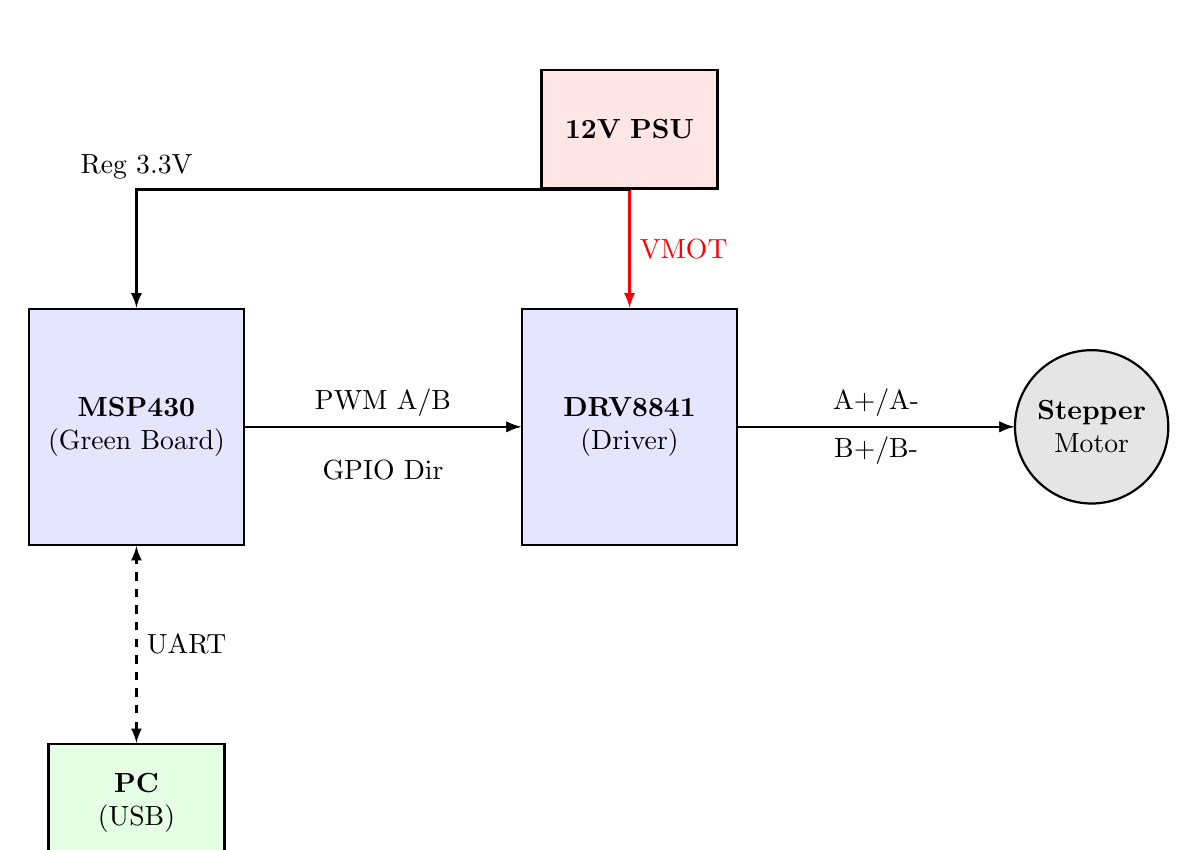
\begin{tikzpicture}[node distance=2.5cm, auto, >=latex, thick]
    % Styles
    \tikzstyle{block} = [rectangle, draw, fill=blue!10, text width=2.5cm, text centered, minimum height=3cm]
    \tikzstyle{motor} = [circle, draw, fill=gray!20, text width=1.5cm, text centered, minimum height=1.5cm]
    \tikzstyle{psu} = [rectangle, draw, fill=red!10, text width=2cm, text centered, minimum height=1.5cm]

    % Nodes
    \node [block] (mcu) {\textbf{MSP430}\\(Green Board)};
    \node [block, right=of mcu, xshift=1cm] (driver) {\textbf{DRV8841}\\(Driver)};
    \node [motor, right=of driver, xshift=1cm] (stepper) {\textbf{Stepper}\\Motor};
    \node [psu, above=of driver, yshift=-1cm] (power) {\textbf{12V PSU}};
    \node [psu, below=of mcu, fill=green!10] (pc) {\textbf{PC}\\(USB)};

    % Connections
    % Power
    \draw[->, red] (power.south) -- (driver.north) node[midway, right] {VMOT};
    \draw[->] (power.south) -| (mcu.north) node[midway, above] {Reg 3.3V};

    % Logic
    \draw[->] (mcu.east) -- (driver.west) node[midway, above] {PWM A/B};
    \draw[->] (mcu.east) -- (driver.west) node[midway, below, yshift=-0.3cm] {GPIO Dir};
    
    % Motor
    \draw[->] (driver.east) -- (stepper.west) node[midway, above] {A+/A-};
    \draw[->] (driver.east) -- (stepper.west) node[midway, below] {B+/B-};
    
    % PC
    \draw[<->, dashed] (pc.north) -- (mcu.south) node[midway, right] {UART};

\end{tikzpicture}
\caption{Electrical Schematic of Stepper Control System}
\label{fig:sch_ex2}
\end{figure}

\textbf{Speed Measurements:}
\begin{itemize}
    \item \textbf{Max No-Load Speed}: [Value] steps/s
    \item \textbf{Max Loaded Speed}: [Value] steps/s
\end{itemize}

\textbf{Discussion:}
The maximum speed is limited by the inductance of the motor coils, which opposes rapid current changes. As speed increases, the current doesn't have enough time to reach the target level within a step period, reducing torque until the motor stalls.

\section{Exercise 3: 2-Axis Control with Dual Stepper Motors}

\subsection{Objective}
To extend the system to 2 axes (X and Y) for a gantry stage. This requires driving a second stepper motor using an external H-bridge driver wired to the PCB.

\subsection{Procedure}

\subsubsection{Gantry Assembly}
The 2-axis gantry was assembled using V-slot aluminum extrusions and timing belts. The procedure followed the standard build provided in the lab manual, with the following key steps:
\begin{enumerate}
    \item \textbf{Frame}: Assembled the base frame using corner brackets and T-nuts.
    \item \textbf{X-Axis}: Mounted the X-axis carriage and belt drive.
    \item \textbf{Y-Axis}: Mounted the Y-axis extrusion on top of the X-carriage.
    \item \textbf{Pen Holder}: Uniquely, we designed and 3D printed a custom pen holder that attaches to the Y-axis slider. This holder uses a interference fit to secure a Sharpie marker, ensuring rigid contact with the paper during drawing operations.
\end{enumerate}

\subsubsection{Wiring the Second Motor}
To enable Y-axis control, a second stepper driver (Pololu DRV8825) was wired to the system. Figure \ref{fig:sch_ex3} illustrates the 2-axis connections.

\begin{figure}[H]
\centering
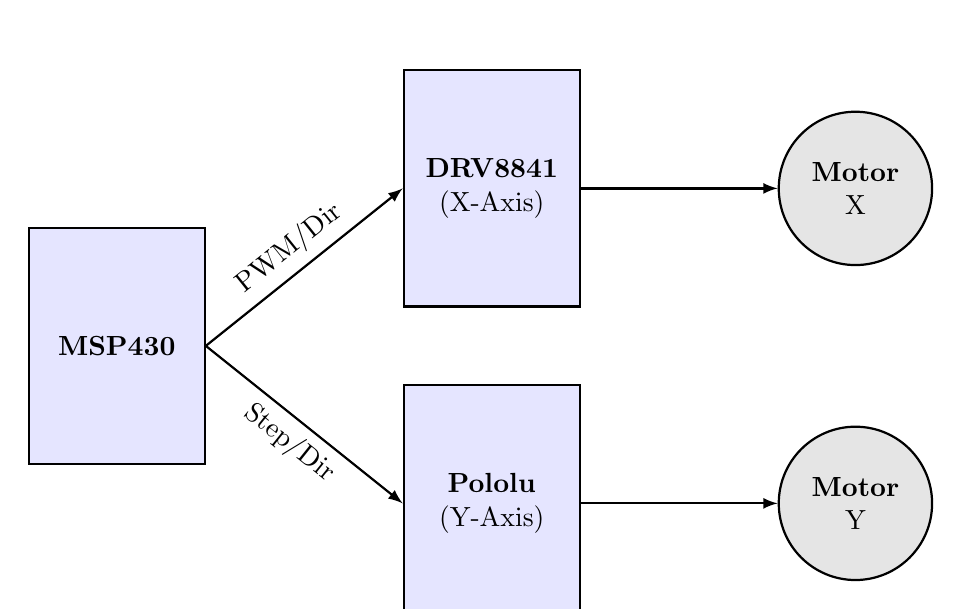
\begin{tikzpicture}[node distance=2.5cm, auto, >=latex, thick]
    \tikzstyle{block} = [rectangle, draw, fill=blue!10, text width=2cm, text centered, minimum height=3cm]
    \tikzstyle{motor} = [circle, draw, fill=gray!20, text width=1.5cm, text centered, minimum height=1.5cm]

    \node [block] (mcu) {\textbf{MSP430}};
    \node [block, right=of mcu, yshift=2cm] (drvX) {\textbf{DRV8841}\\(X-Axis)};
    \node [block, right=of mcu, yshift=-2cm] (drvY) {\textbf{Pololu}\\(Y-Axis)};
    \node [motor, right=of drvX] (motX) {\textbf{Motor}\\X};
    \node [motor, right=of drvY] (motY) {\textbf{Motor}\\Y};
    
    % Connections
    \draw[->] (mcu.east) -- (drvX.west) node[midway, above, sloped] {PWM/Dir};
    \draw[->] (mcu.east) -- (drvY.west) node[midway, below, sloped] {Step/Dir};
    \draw[->] (drvX.east) -- (motX.west);
    \draw[->] (drvY.east) -- (motY.west);
\end{tikzpicture}
\caption{2-Axis Control Wiring Diagram}
\label{fig:sch_ex3}
\end{figure}

\subsubsection{Coordinated Motion Control (Firmware)}
To draw straight lines and complex shapes, the X and Y axes must move in sync. We implemented a simplified Digital Differential Analyzer (DDA) algorithm in the firmware.

\textbf{Firmware Logic:}
The `Timer\_A1\_ISR` function serves as the central tick for motion.
\begin{enumerate}
    \item \textbf{Accumulators}: We maintain `acc\_x` and `acc\_y`.
    \item \textbf{Step Decision}: At every interrupt, we add the target delta ($\Delta X, \Delta Y$) to the accumulators.
    \item \textbf{Threshold}: If an accumulator exceeds `total\_steps`, a step is issued to that motor, and `total\_steps` is subtracted.
\end{enumerate}
This ensures that the ratio of X steps to Y steps is constant, producing a straight line.

\begin{lstlisting}[language=C]
// DDA Algorithm in Timer_A1_ISR
acc_x += delta_x;
acc_y += delta_y;

if (acc_x >= total_steps_needed) {
    motor1_state = (motor1_state + step_x_inc) & 0x07;
    step_motor1(motor1_state);
    acc_x -= total_steps_needed;
}
// Repeat for Y...
\end{lstlisting}

\subsection{Software Interface Features}
The C\# application provides a comprehensive dashboard:
\begin{itemize}
    \item \textbf{Connection Panel}: Serial port selection and connect/disconnect.
    \item \textbf{Manual Control}: Slider for variable speed (1-100\%), Buttons for single stepping.
    \item \textbf{Gantry Control}: Input fields for X/Y coordinates (cm) and "Move" button.
    \item \textbf{Image Processing}:
    \begin{itemize}
        \item \textbf{Canvas}: Displays the loaded image and computed path.
        \item \textbf{Import}: Loads JPG/PNG.
        \item \textbf{Process}: Runs Sobel edge detection and Nearest Neighbor sorting.
        \item \textbf{Draw}: Sends the point stream to the robot.
    \end{itemize}
\end{itemize}

\subsection{Image Processing Results \& Critique}
The "Image to Drawing" feature successfully identified edges and generated a path, but the physical result was mixed. The bitmaps were recognizable, but the drawing quality suffered due to several factors:

\begin{itemize}
    \item \textbf{Z-Axis}: We lacked a Z-axis servo to lift the pen between strokes. This resulted in "travel lines" connecting distinct parts of the drawing, cluttering the image.
    \item \textbf{Precision}: The nearest-neighbor path optimization is greedy and often chose sub-optimal routes, increasing drawing time and error accumulation.
    \item \textbf{Mechanical}: The pen holder, while rigid, had no suspension. Variations in table height caused the pen to skip or dig into the paper.
\end{itemize}

\textbf{Future Improvements:}
\begin{enumerate}
    \item Add a servo to lift the pen.
    \item Implement microstepping (1/16 or 1/32) to smooth out the lines.
    \item Use a vector-based approach (SVG) instead of raster edge detection for cleaner lines.
\end{enumerate}

\subsection{Results}
We tested the gantry by drawing standard shapes (Square, Diamond, Triangle) and a complex "Creative Shape" (imported image).

\imageplaceholder{Standard Shapes Plot}{Insert photo of the paper with the 6 test points/lines drawn.}

\imageplaceholder{Creative Shape Plot}{Insert photo of the creative shape drawn by the gantry.}

\imageplaceholder{Creative Shape Design Overlay}{Insert photo of the drawn shape with the intended design overlaid for comparison.}

\textbf{Discussion on Accuracy:}
Deviations between the design and the result can be attributed to:
\begin{itemize}
    \item \textbf{Backlash}: Play in the belt/pulley system caused circle endpoints to not perfectly meet.
    \item \textbf{Vibration}: At high speeds, the gantry frame resonance caused some line waviness.
    \item \textbf{Resolution}: The standard 200 step/rev motor + DDA rounding errors limit the finest detail to approx 0.2mm.
\end{itemize}

\section{Conclusion}
This lab successfully demonstrated the complete process of building a mechatronic controller, from soldering the PCB to implementing low-level motor control firmware and high-level PC software. The final 2-axis gantry system was able to draw complex shapes, validating the integration of all subsystems.

\newpage
\newpage
\appendix
\section{Exercise 2 Code}
\subsection{Microcontroller Firmware}
(Note: Exercise 2 functionality was integrated into the Exercise 3 firmware below.)

\subsection{PC Interface (C\#)}
\lstinputlisting[language=C, caption=StepperCommander.cs]{code/ex2/StepperCommander.cs}
\lstinputlisting[language=C, caption=Form1.cs]{code/ex2/Form1.cs}

\section{Exercise 3 Code}
\subsection{Microcontroller Firmware}
\lstinputlisting[language=C, caption=main.c]{code/ex3/main.c}

\subsection{PC Interface (C\#)}
\lstinputlisting[language=C, caption=MainWindow.xaml.cs]{code/ex3/MainWindow.xaml.cs}

\end{document}
